\documentclass{standalone}
\usepackage{tikz}
\usetikzlibrary{patterns, positioning}
\usepackage[sfdefault]{ClearSans} %% option 'sfdefault' activates Clear Sans as the default text font
\usepackage[T1]{fontenc}

\begin{document}
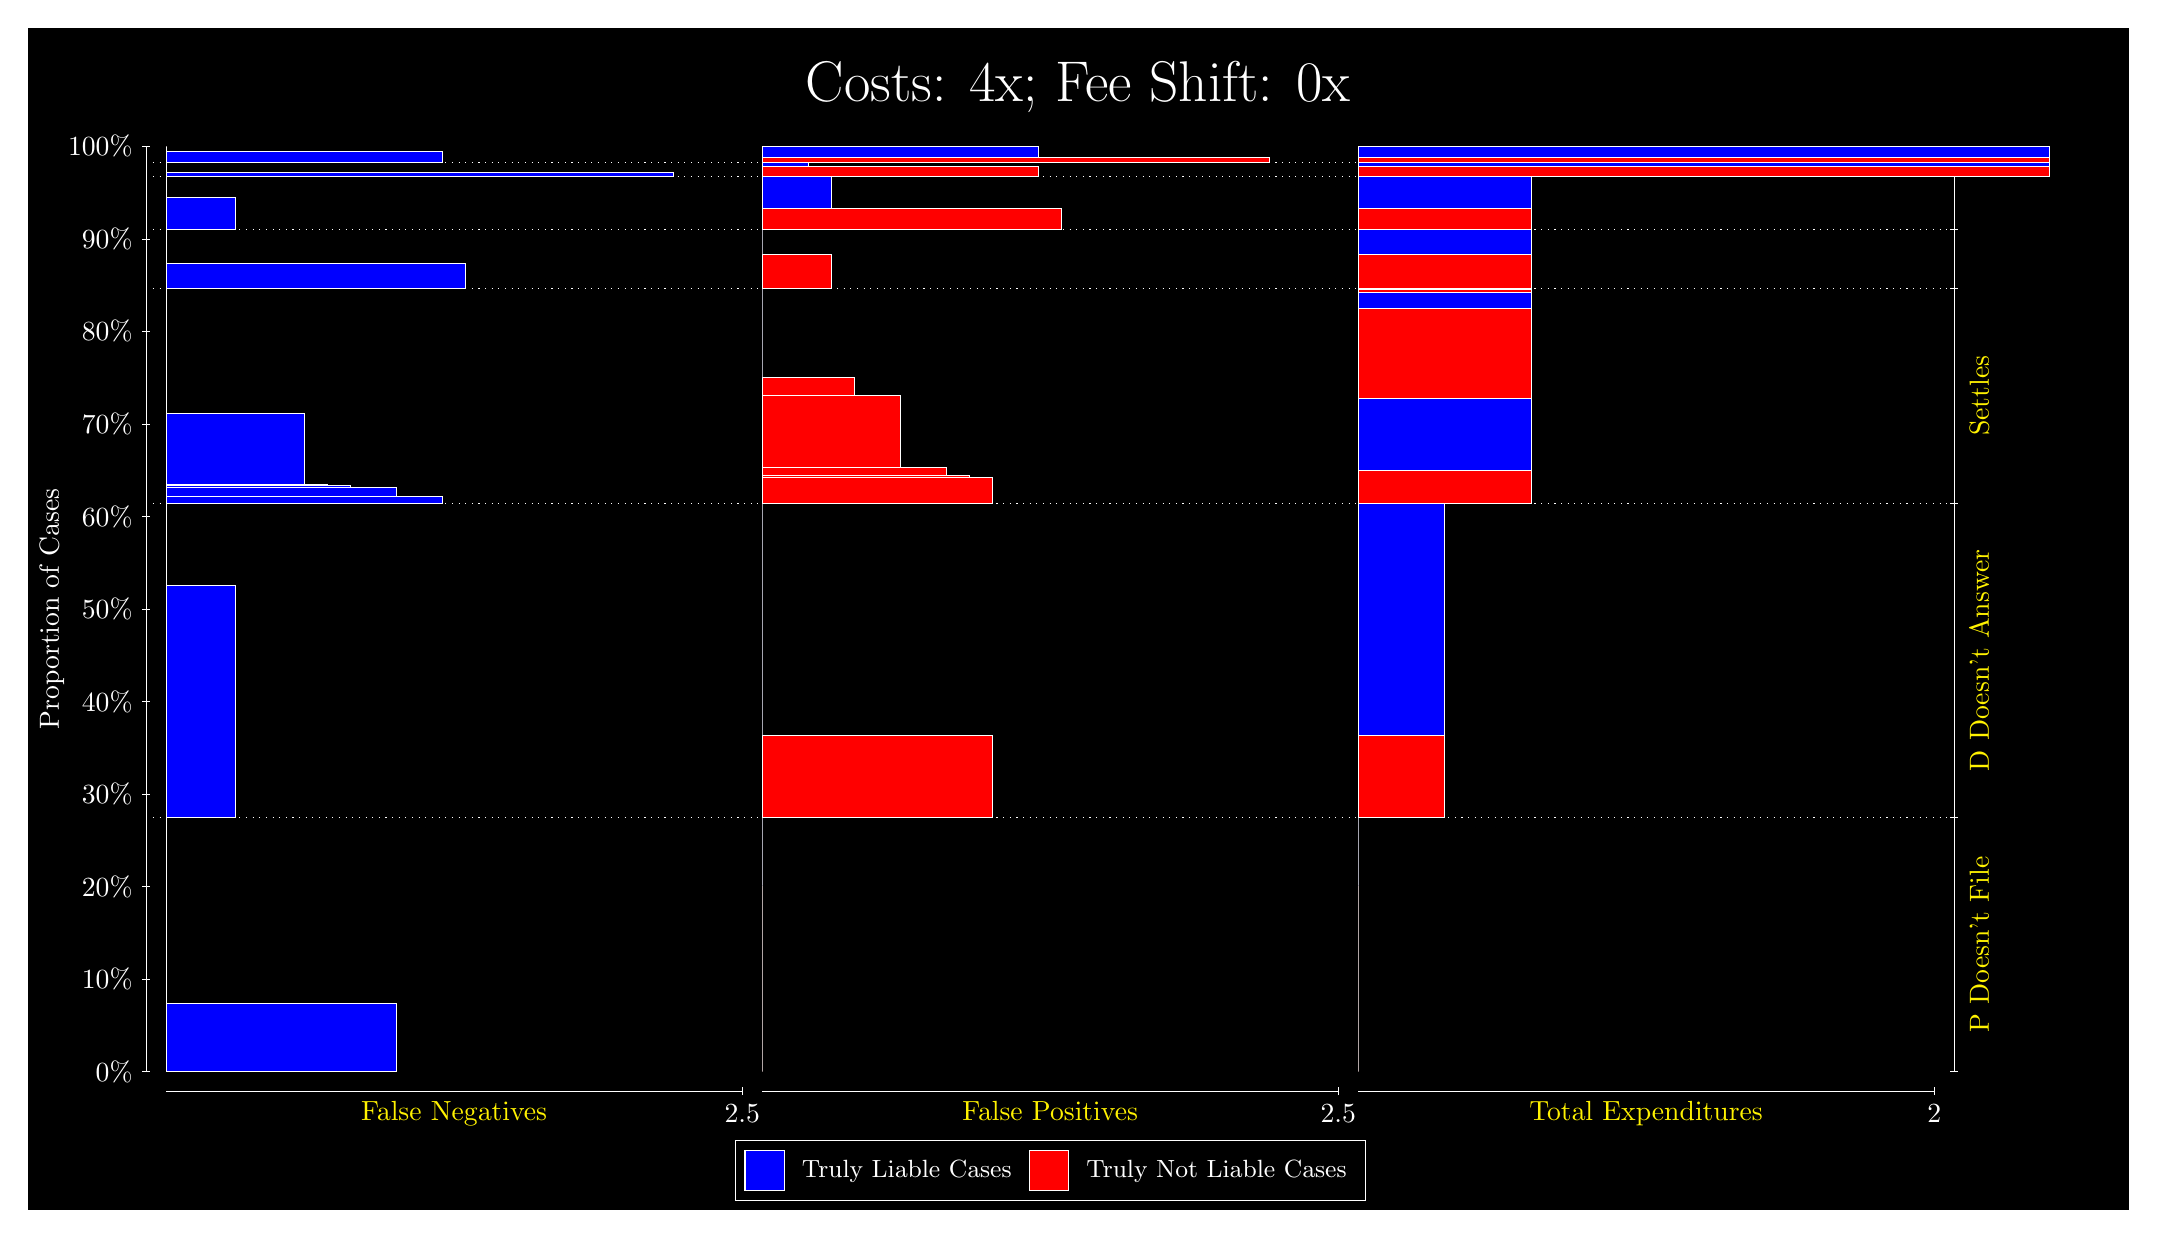
\begin{tikzpicture}
\draw[fill=black] (0,0) rectangle (26.667,15);
\draw[text=white] (0,13.5) rectangle (26.667,15) node[midway] {\huge Costs: 4x; Fee Shift: 0x};
\draw[white, very thin] (1.5,1.75) -- (1.5,13.5);
\node[rotate=90, text=white, anchor=center] at (0.3, 7.625) {Proportion of Cases};
\draw[white, very thin] (1.45,1.75) -- (1.55,1.75);
\node[text=white, anchor=east] at (1.45, 1.75) {0\%};
\draw[white, very thin] (1.45,2.925) -- (1.55,2.925);
\node[text=white, anchor=east] at (1.45, 2.925) {10\%};
\draw[white, very thin] (1.45,4.1) -- (1.55,4.1);
\node[text=white, anchor=east] at (1.45, 4.1) {20\%};
\draw[white, very thin] (1.45,5.275) -- (1.55,5.275);
\node[text=white, anchor=east] at (1.45, 5.275) {30\%};
\draw[white, very thin] (1.45,6.45) -- (1.55,6.45);
\node[text=white, anchor=east] at (1.45, 6.45) {40\%};
\draw[white, very thin] (1.45,7.625) -- (1.55,7.625);
\node[text=white, anchor=east] at (1.45, 7.625) {50\%};
\draw[white, very thin] (1.45,8.8) -- (1.55,8.8);
\node[text=white, anchor=east] at (1.45, 8.8) {60\%};
\draw[white, very thin] (1.45,9.975) -- (1.55,9.975);
\node[text=white, anchor=east] at (1.45, 9.975) {70\%};
\draw[white, very thin] (1.45,11.15) -- (1.55,11.15);
\node[text=white, anchor=east] at (1.45, 11.15) {80\%};
\draw[white, very thin] (1.45,12.325) -- (1.55,12.325);
\node[text=white, anchor=east] at (1.45, 12.325) {90\%};
\draw[white, very thin] (1.45,13.5) -- (1.55,13.5);
\node[text=white, anchor=east] at (1.45, 13.5) {100\%};

\draw[white, very thin] (24.457,1.75) -- (24.457,13.5);
\draw[white, very thin] (24.407,1.75) -- (24.507,1.75);
\node[anchor=west] at (24.407, 1.75) {};
\draw[white, very thin] (24.407,4.9762) -- (24.507,4.9762);
\node[anchor=west] at (24.407, 4.9762) {};
\draw[white, very thin] (24.407,8.9679) -- (24.507,8.9679);
\node[anchor=west] at (24.407, 8.9679) {};
\draw[white, very thin] (24.407,11.7) -- (24.507,11.7);
\node[anchor=west] at (24.407, 11.7) {};
\draw[white, very thin] (24.407,12.448) -- (24.507,12.448);
\node[anchor=west] at (24.407, 12.448) {};
\draw[white, very thin] (24.407,13.117) -- (24.507,13.117);
\node[anchor=west] at (24.407, 13.117) {};
\draw[white, very thin] (24.407,13.299) -- (24.507,13.299);
\node[anchor=west] at (24.407, 13.299) {};
\draw[white, very thin] (24.407,13.5) -- (24.507,13.5);
\node[anchor=west] at (24.407, 13.5) {};

\draw[white, very thin, fill=blue] (1.75,1.75) rectangle (4.6775,2.6146);
\draw[white, very thin, fill=red] (1.75,2.6146) rectangle (1.75,4.9762);
\draw[white, very thin, fill=blue] (1.75,4.9762) rectangle (2.6283,7.929);
\draw[white, very thin, fill=red] (1.75,7.929) rectangle (1.75,8.9679);
\draw[white, very thin, fill=blue] (1.75,8.9679) rectangle (5.2631,9.0559);
\draw[white, very thin, fill=blue] (1.75,9.0559) rectangle (4.6775,9.1713);
\draw[white, very thin, fill=blue] (1.75,9.1713) rectangle (4.092,9.1936);
\draw[white, very thin, fill=blue] (1.75,9.1936) rectangle (3.7993,9.2122);
\draw[white, very thin, fill=blue] (1.75,9.2122) rectangle (3.5065,10.104);
\draw[white, very thin, fill=red] (1.75,10.104) rectangle (1.75,11.7);
\draw[white, very thin, fill=blue] (1.75,11.7) rectangle (5.5558,12.021);
\draw[white, very thin, fill=red] (1.75,12.021) rectangle (1.75,12.448);
\draw[white, very thin, fill=blue] (1.75,12.448) rectangle (2.6283,12.848);
\draw[white, very thin, fill=red] (1.75,12.848) rectangle (1.75,13.117);
\draw[white, very thin, fill=blue] (1.75,13.117) rectangle (8.1906,13.174);
\draw[white, very thin, fill=red] (1.75,13.174) rectangle (1.75,13.299);
\draw[white, very thin, fill=blue] (1.75,13.299) rectangle (5.2631,13.443);
\draw[white, very thin, fill=red] (1.75,13.443) rectangle (1.75,13.5);
\draw[white, very thin, fill=red] (9.3189,1.75) rectangle (9.3189,4.1116);
\draw[white, very thin, fill=blue] (9.3189,4.1116) rectangle (9.3189,4.9762);
\draw[white, very thin, fill=red] (9.3189,4.9762) rectangle (12.246,6.015);
\draw[white, very thin, fill=blue] (9.3189,6.015) rectangle (9.3189,8.9679);
\draw[white, very thin, fill=red] (9.3189,8.9679) rectangle (12.246,9.2945);
\draw[white, very thin, fill=red] (9.3189,9.2945) rectangle (11.954,9.3281);
\draw[white, very thin, fill=red] (9.3189,9.3281) rectangle (11.661,9.4207);
\draw[white, very thin, fill=red] (9.3189,9.4207) rectangle (11.075,10.333);
\draw[white, very thin, fill=red] (9.3189,10.333) rectangle (10.49,10.564);
\draw[white, very thin, fill=blue] (9.3189,10.564) rectangle (9.3189,11.7);
\draw[white, very thin, fill=red] (9.3189,11.7) rectangle (10.197,12.128);
\draw[white, very thin, fill=blue] (9.3189,12.128) rectangle (9.3189,12.448);
\draw[white, very thin, fill=red] (9.3189,12.448) rectangle (13.125,12.718);
\draw[white, very thin, fill=blue] (9.3189,12.718) rectangle (10.197,13.117);
\draw[white, very thin, fill=red] (9.3189,13.117) rectangle (12.832,13.242);
\draw[white, very thin, fill=blue] (9.3189,13.242) rectangle (9.9044,13.299);
\draw[white, very thin, fill=red] (9.3189,13.299) rectangle (15.759,13.355);
\draw[white, very thin, fill=blue] (9.3189,13.355) rectangle (12.832,13.5);
\draw[white, very thin, fill=red] (16.888,1.75) rectangle (16.888,4.1116);
\draw[white, very thin, fill=blue] (16.888,4.1116) rectangle (16.888,4.9762);
\draw[white, very thin, fill=red] (16.888,4.9762) rectangle (17.986,6.015);
\draw[white, very thin, fill=blue] (16.888,6.015) rectangle (17.986,8.9679);
\draw[white, very thin, fill=red] (16.888,8.9679) rectangle (19.083,9.3872);
\draw[white, very thin, fill=blue] (16.888,9.3872) rectangle (19.083,10.301);
\draw[white, very thin, fill=red] (16.888,10.301) rectangle (19.083,11.444);
\draw[white, very thin, fill=blue] (16.888,11.444) rectangle (19.083,11.648);
\draw[white, very thin, fill=red] (16.888,11.648) rectangle (19.083,11.681);
\draw[white, very thin, fill=blue] (16.888,11.681) rectangle (19.083,11.7);
\draw[white, very thin, fill=red] (16.888,11.7) rectangle (19.083,12.128);
\draw[white, very thin, fill=blue] (16.888,12.128) rectangle (19.083,12.448);
\draw[white, very thin, fill=red] (16.888,12.448) rectangle (19.083,12.718);
\draw[white, very thin, fill=blue] (16.888,12.718) rectangle (19.083,13.117);
\draw[white, very thin, fill=red] (16.888,13.117) rectangle (25.67,13.242);
\draw[white, very thin, fill=blue] (16.888,13.242) rectangle (25.67,13.299);
\draw[white, very thin, fill=red] (16.888,13.299) rectangle (25.67,13.355);
\draw[white, very thin, fill=blue] (16.888,13.355) rectangle (25.67,13.5);
\draw[white, dotted] (1.5,4.9762) -- (24.457,4.9762);
\draw[white, dotted] (1.5,8.9679) -- (24.457,8.9679);
\draw[white, dotted] (1.5,11.7) -- (24.457,11.7);
\draw[white, dotted] (1.5,12.448) -- (24.457,12.448);
\draw[white, dotted] (1.5,13.117) -- (24.457,13.117);
\draw[white, dotted] (1.5,13.299) -- (24.457,13.299);
\draw[white, very thin] (1.75,1.5) -- (9.0689,1.5);
\node[text=yellow, anchor=north] at (5.4094, 1.5) {False Negatives};
\draw[white, very thin] (9.0689,1.45) -- (9.0689,1.55);
\node[text=white, anchor=north] at (9.0689, 1.45) {2.5};

\draw[white, very thin] (9.3189,1.5) -- (16.638,1.5);
\node[text=yellow, anchor=north] at (12.978, 1.5) {False Positives};
\draw[white, very thin] (16.638,1.45) -- (16.638,1.55);
\node[text=white, anchor=north] at (16.638, 1.45) {2.5};

\draw[white, very thin] (16.888,1.5) -- (24.207,1.5);
\node[text=yellow, anchor=north] at (20.547, 1.5) {Total Expenditures};
\draw[white, very thin] (24.207,1.45) -- (24.207,1.55);
\node[text=white, anchor=north] at (24.207, 1.45) {2};

\node[text=yellow, centered, rotate=90] at (24.777, 3.3631) {P Doesn't File};
\node[text=yellow, centered, rotate=90] at (24.777, 6.972) {D Doesn't Answer};
\node[text=yellow, centered, rotate=90] at (24.777, 10.334) {Settles};





\draw (12.978300999999998,1.5) node[draw=none] (baseCoordinate) {};
\begin{scope}[align=center]
        \matrix[scale=0.5, draw=white, below=0.5cm of baseCoordinate, nodes={draw}, column sep=0.1cm]{
            \node[rectangle, draw, minimum width=0.5cm, minimum height=0.5cm, fill=blue] {}; &
            \node[draw=none, font=\small, text=white] (B) {Truly Liable Cases}; &
            \node[rectangle, draw, minimum width=0.5cm, minimum height=0.5cm, fill=red] {}; &
            \node[draw=none, font=\small, text=white] (B) {Truly Not Liable Cases}; \\
            };
\end{scope}

\end{tikzpicture}
\end{document}